\section{Query e Indici}

\subsection{Query}
\begin{enumerate}
\item[Query 1)] Restituisce Nome,Cognome,CF di manutentori che hanno eseguito almeno una manutenzione nel mese corrente. Viene inoltre mostrata la durata in un formato ore\_minuti di tale manutenzione affinche' il manutentore possa essere retribuito in base al tempo dedicato a tali manutenzioni.\\

\lstinputlisting[language=SQL, firstline=7, lastline=11]{Query.sql}

\begin{center}
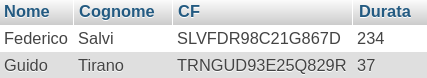
\includegraphics[scale=0.6]{Query1}
\end{center}

Viene dunque mostrato che Federico Salvi ha eseguito una o piu' manutenzioni nell'arco del mese corrente per una durata di 2:34 ore. Analogamente viene mostrato quanto tempo ha lavorato ad una o piu' manutenzioni Guido Tirano.\\

\item[Query 2)] Restituisce Nome, Cognome e Email di tutti i clienti che non hanno mai effettuato un acquisto o che non lo hanno effettuato in particolare negli ultimi 6 mesi. Questo permette poi al negozio di inviare delle email promozionali a tali clienti per invogliarli a procedere con un acquisto.\\

\lstinputlisting[language=SQL, firstline=20, lastline=27]{Query.sql}

\begin{center}
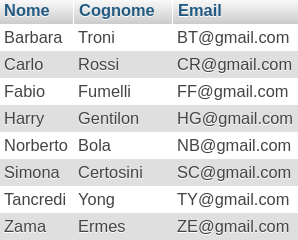
\includegraphics[scale=0.6]{Query2}
\end{center}

Con la query annidata si vanno a ricercare tutti i clienti che \textbf{hanno} effettuato un acquisto negli ultimi 6 mesi (estraendo le date degli acquisti e confrontandole con quella corrente), successivamente si vanno a scegliere tutti gli ID di clienti che \textbf{non} sono presenti in tale selezione.\\

\item[Query 3)]Per ogni negozio restituisce ID, Nome e Produttore dei componenti venduti piu' di una volta da tale negozio.\\

\lstinputlisting[language=SQL, firstline=37, lastline=43]{Query.sql}

\begin{center}
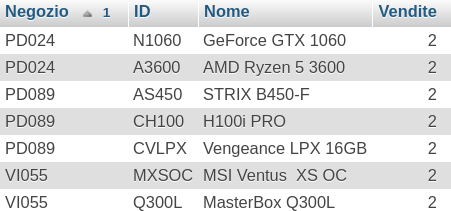
\includegraphics[scale=0.6]{Query3}
\end{center}

\item[Query 4)] Ritorna ID, Indirizzo dei negozi, insieme alla media degli stipendi recepiti dai dipendenti e al totale degli acquisti registrati per ogni negozio appartenente alla catena.\\

\lstinputlisting[language=SQL, firstline=49, lastline=60]{Query.sql}

\begin{center}
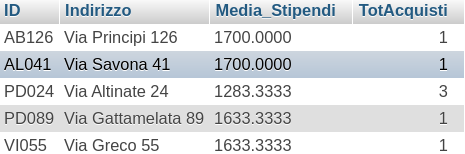
\includegraphics[scale=0.6]{Query4}
\end{center}

La query e' realizzata mediante l'utilizzo di una vista di supporto che seleziona il numero totale di acquisti registrati da ciascun negozio.  La query successivamente utilizza questa vista per restituire il totale degli acqusiti, oltre alla media degli stipendi per ogni esercizio commericale.\\

\item[Query 5)] Restituisce i componenti relativi all'acquisto '17 0000003' che non sono presenti in magazzino e che dovranno dunque essere ordinati.\\

\lstinputlisting[language=SQL, firstline=70, lastline=77]{Query.sql}

\begin{center}
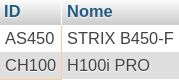
\includegraphics[scale=0.6]{Query5}
\end{center}

La sotto-query prende in esame tutti i componenti contenuti nel magazzino corrispondente al negozio dove e' stato registrato l'acquisto. Successivamente si vanno a selezionare gli ID dei componenti che formano l'acquisto, che pero' non sono riportati dalla sotto-query e che quindi non sono presenti in magazzino.\\

\item[Query 6)] Restituisce ID, Nome e Prezzo di tutti i componenti registrati che risultano avere un prezzo minore della media del totale degli acquisti di componenti formati da un singolo articolo. \\

\lstinputlisting[language=SQL, firstline =83, lastline =97]{Query.sql}

Anche questa query (analogamente a quanto succede nella numero 4) si serve di una vista. Tale vista seleziona gli acquisti formati da un singolo componente e ne riporta anche il totale. Questo per permettere alla query di confrontare il prezzo di tutti i componenti registrati con la media dei totali riportati dalla vista(quindi di ogni acquisto singolo).\\
L'output della query per mancanza di spazio viene riportato interamente nella pagina seguente.\\
\begin{center}
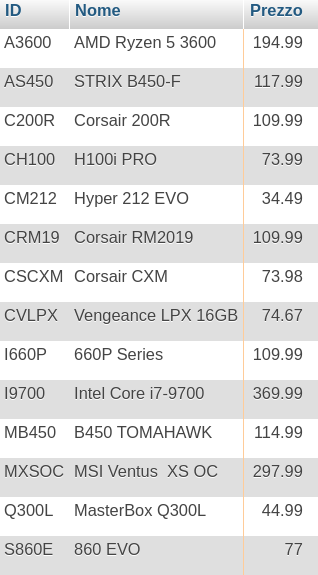
\includegraphics[scale=0.6]{Query6}
\end{center}

\end{enumerate}


\subsection{Indici} 

Ipotizzando che il database di \textbf{Hardware House} sia di dimensioni molto elevate e in particolare:
\begin{itemize}
\item La tabella \textbf{Componente} contenga al suo interno molte tuple
\item I componenti nuovi introdotti nel mercato siano in misura non troppo elevata
\item La ricerca dei componenti e' un' operazione svolta con una frequenza sufficientemente alta
\end{itemize}

Si considera l'indicizzazione della tabella \textbf{Componente} al fine di velocizzare le operazioni di ricerca che coinvolgono quest'ultimi.\\ 
In particolare la maggior parte delle ricerche interessa maggiormente la tipologia del componente, piu' che il suo identificativo o il suo nome, dunque l'indicizzazione averra' non su l'intera tabella ma sull' attributo \textbf{Tipo}.\\
Il codice che interessa la creazione degli indici e' il seguente:\\

\lstinputlisting[language=SQL, firstline = 101, lastline = 101]{Query.sql}


